Welcome to the third assignment! During this assignment, you will practice your
math skills in an environment more similar to the one that you will face during
the course assessment. Although the questions will not be the same, they will
follow the same structure and you will have to solve the exercises using the
Dirac notation or matrix--vector multiplication.

Together with this assignment, you will find the \LaTeX { template} for you to
use when solving the exercises and writing down your answers. Remember to
upload a single pdf file with the full development of the assignment and the
answers.

\begin{question}
Are the quantum states $\ket{\psi_{1}} = \ket{00}$ and $\ket{\psi_{2}} = \ket{++}$ mutually orthogonal?
\label{qst:assignment3_1}
\end{question}
{\small
\texttt{Write down your solution here:}
\begin{equation*}
  \begin{split}
  \text{The two states are mutually orthogonal when the inner product is 0.}\\
  \rightarrow\ket{++}=\ket{+}\otimes\ket{+}=\frac{1}{\sqrt{2}}(\ket{0}+\ket{1}\otimes\frac{1}{\sqrt{2}}(\ket{0}+\ket{1})
  \\
  \rightarrow\ket{++}=\frac{1}{2}(\ket{00}+\ket{01}+\ket{10}+\ket{11}
  \\
  \rightarrow\bra{00}\ket{++}=\ket{00}\cdot\frac{1}{2}(\ket{00}+\ket{01}+\ket{10}+\ket{11}
  \\
  \rightarrow\bra{00}\ket{++}=\frac{1}{2}(\bra{00}\ket{00}+\bra{00}\ket{01}+\bra{00}\ket{10}+\bra{00}\ket{11}
  \\
  \rightarrow\bra{00}\ket{++}=\frac{1}{2}(1+0+0+0)=\frac{1}{2}\neq0
  \\
  \text{The states are mutually orthogonal.}
  \end{split}
\end{equation*}}
\vspace{0.1cm}

\begin{question}
Let $\ket{\psi} = \frac{4}{5} \ket{00} + \frac{2}{5} \ket{01} + \frac{2}{5} \ket{10} + \frac{1}{5} \ket{11}$. What is the probability of obtaining $M(q_{1} = 0)$ when measuring the system?
\label{qst:assignment3_2}
\end{question}
{\small
\texttt{Write down your solution here:}
\begin{equation*}
  \begin{split}
    \Prob{q_{1} = 0} \rightarrow (\frac{4}{5})^2\ket{00}+(\frac{2}{5})^2\ket{01}=\frac{16}{25}+\frac{4}{25}=\frac{20}{25}=\frac{4}{5}=80\%
  \end{split}
\end{equation*}}
\vspace{0.1cm}

\begin{question}
What is the resulting transformation matrix $T_{1}$ when applied the following operation $T_{1} = Y \otimes S$
\label{qst:assignment3_3}
\end{question}
{\small
\texttt{Write down your solution here:}
\begin{equation*}
  \begin{split}
    T_{1} &=
    \begin{bmatrix}
        0&-i \\ i&0
    \end{bmatrix}
    \otimes
    \begin{bmatrix}
        1&0 \\ 0&i
    \end{bmatrix}
    =
    \begin{bmatrix}
        0&0&-i&0 \\
        0&0&0&1 \\
        i&0&0&0 \\
        0&-1&0&0
    \end{bmatrix}
  \end{split}
\end{equation*}}
\vspace{0.1cm}

\begin{figure}[t]
  \centerline{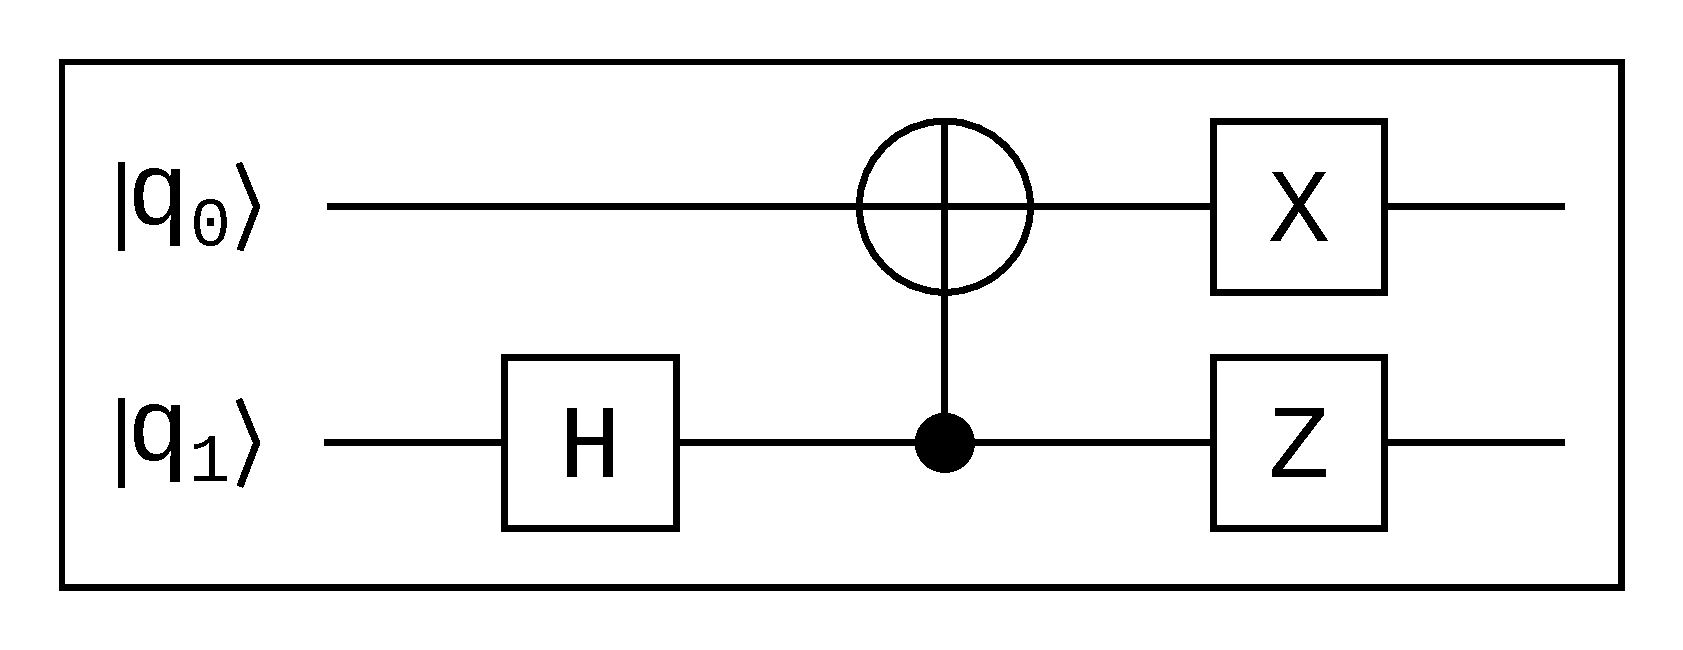
\includegraphics[scale=0.25]{img/qci_a3_question4.ps}}
  \caption{An arbitrary quantum circuit.}
  \label{fig:circuit2}
\end{figure}

\begin{question}
Consider the quantum circuit presented in Figure~\ref{fig:circuit2} and assume $\ket{q_{1}} = \ket{1}$ and $\ket{q_{0}} = \ket{0}$; hence, $\ket{\psi_{in}} = \ket{10}$. Determine, by using the matrix--vector multiplication, what is the state vector of the quantum circuit just before the measurement?
\label{qst:assignment3_4}
\end{question}
{\small
\texttt{Write down your solution here:}
\begin{equation*}
  \begin{split}
  I\ket{Q_{0}}=
  \begin{bmatrix}
      1&0\\0&1
  \end{bmatrix}
  \begin{bmatrix}
      1\\0
  \end{bmatrix}
  =
  \begin{bmatrix}
      1\\0
  \end{bmatrix}
  \\
  H\ket{Q_{1}}=\frac{1}{\sqrt{2}}
  \begin{bmatrix}
      1&1\\1&-1
  \end{bmatrix}
  \begin{bmatrix}
      0\\1
  \end{bmatrix}
  =\frac{1}{\sqrt{2}}
  \begin{bmatrix}
      1\\-1
  \end{bmatrix}
  \\
  \ket{\psi}=\frac{1}{\sqrt{2}}(
  \begin{bmatrix}
      1\\0
  \end{bmatrix}
  \otimes
  \begin{bmatrix}
      1\\0
  \end{bmatrix}
  -
  \begin{bmatrix}
      1\\-1
  \end{bmatrix}
  \otimes
  \begin{bmatrix}
      1\\0
  \end{bmatrix}
  )=
  \begin{bmatrix}
      1&0\\0&0
  \end{bmatrix}
  -
  \begin{bmatrix}
      1&0\\-1&0
  \end{bmatrix}
  =
  \begin{bmatrix}
      0&0\\-1&0
  \end{bmatrix}
  \\=
  \frac{1}{\sqrt{2}}(\ket{00}-\ket{10})\\
  \text CNOT_{1,0} = \frac{1}{\sqrt{2}}(\ket{00}-\ket{11})\\
  \\
  \text XQ_{0}=
  \begin{bmatrix}
      0&1\\1&0
  \end{bmatrix}
  \begin{bmatrix}
      0\\1
  \end{bmatrix}
  \bigwedge
  \begin{bmatrix}
      0&1\\1&0
  \end{bmatrix}
  \begin{bmatrix}
      1\\0
  \end{bmatrix}
  =
  \begin{bmatrix}
      1\\0
  \end{bmatrix}
  \bigwedge
  \begin{bmatrix}
      0\\1
  \end{bmatrix}
  =
  (\ket{01}-\ket{10})
  \\
  \text ZQ_{1}=
  \begin{bmatrix}
      1&0\\0&-1
  \end{bmatrix}
  \begin{bmatrix}
      1\\0
  \end{bmatrix}
  =
  \begin{bmatrix}
      1\\0
  \end{bmatrix}
  \bigwedge
  \begin{bmatrix}
      1&0\\0&-1
  \end{bmatrix}
  \begin{bmatrix}
      0\\1
  \end{bmatrix}
  =
  \begin{bmatrix}
      0\\-1
  \end{bmatrix}
  \\
  \\
  \text {Which results in:}\\
  \ket{\psi}=\ket{01}-\ket{10}
  \end{split}
\end{equation*}}
\vspace{0.1cm}

\begin{question}
Consider the quantum circuit presented in Figure~\ref{fig:circuit2} and assume $\ket{q_{1}} = \ket{0}$ and $\ket{q_{0}} = \ket{1}$; hence, $\ket{\psi_{in}} = \ket{01}$. Determine, by using the Dirac notation, what is the state vector of the quantum circuit just before the measurement?
\label{qst:assignment3_5}
\end{question}
{\small
\texttt{Write down your solution here:}
\begin{equation*}
  \begin{split}
      \text H\ket{q_{1}}=\frac{1}{\sqrt{2}}(\ket{0}+\ket{1})
      \\
      \ket{q_{1}}+\ket{q_{0}}=\frac{1}{\sqrt{2}}(\ket{01}+\ket{11})\\
      \text CNOT_{1,0}=\frac{1}{\sqrt{2}}(\ket{01}+\ket{10}\\
      \text Xq_{0} = \frac{1}{\sqrt{2}}(\ket{00}+\ket{11}\\
      \text Zq_{1} = \frac{1}{\sqrt{2}}(\ket{00}-\ket{11}\\
      \text {Final state} = \ket{\psi_{out}}=\frac{1}{\sqrt{2}}(\ket{00}-\ket{11}\\
  \end{split}
\end{equation*}}
\vspace{0.1cm}

\begin{figure}[t]
  \centerline{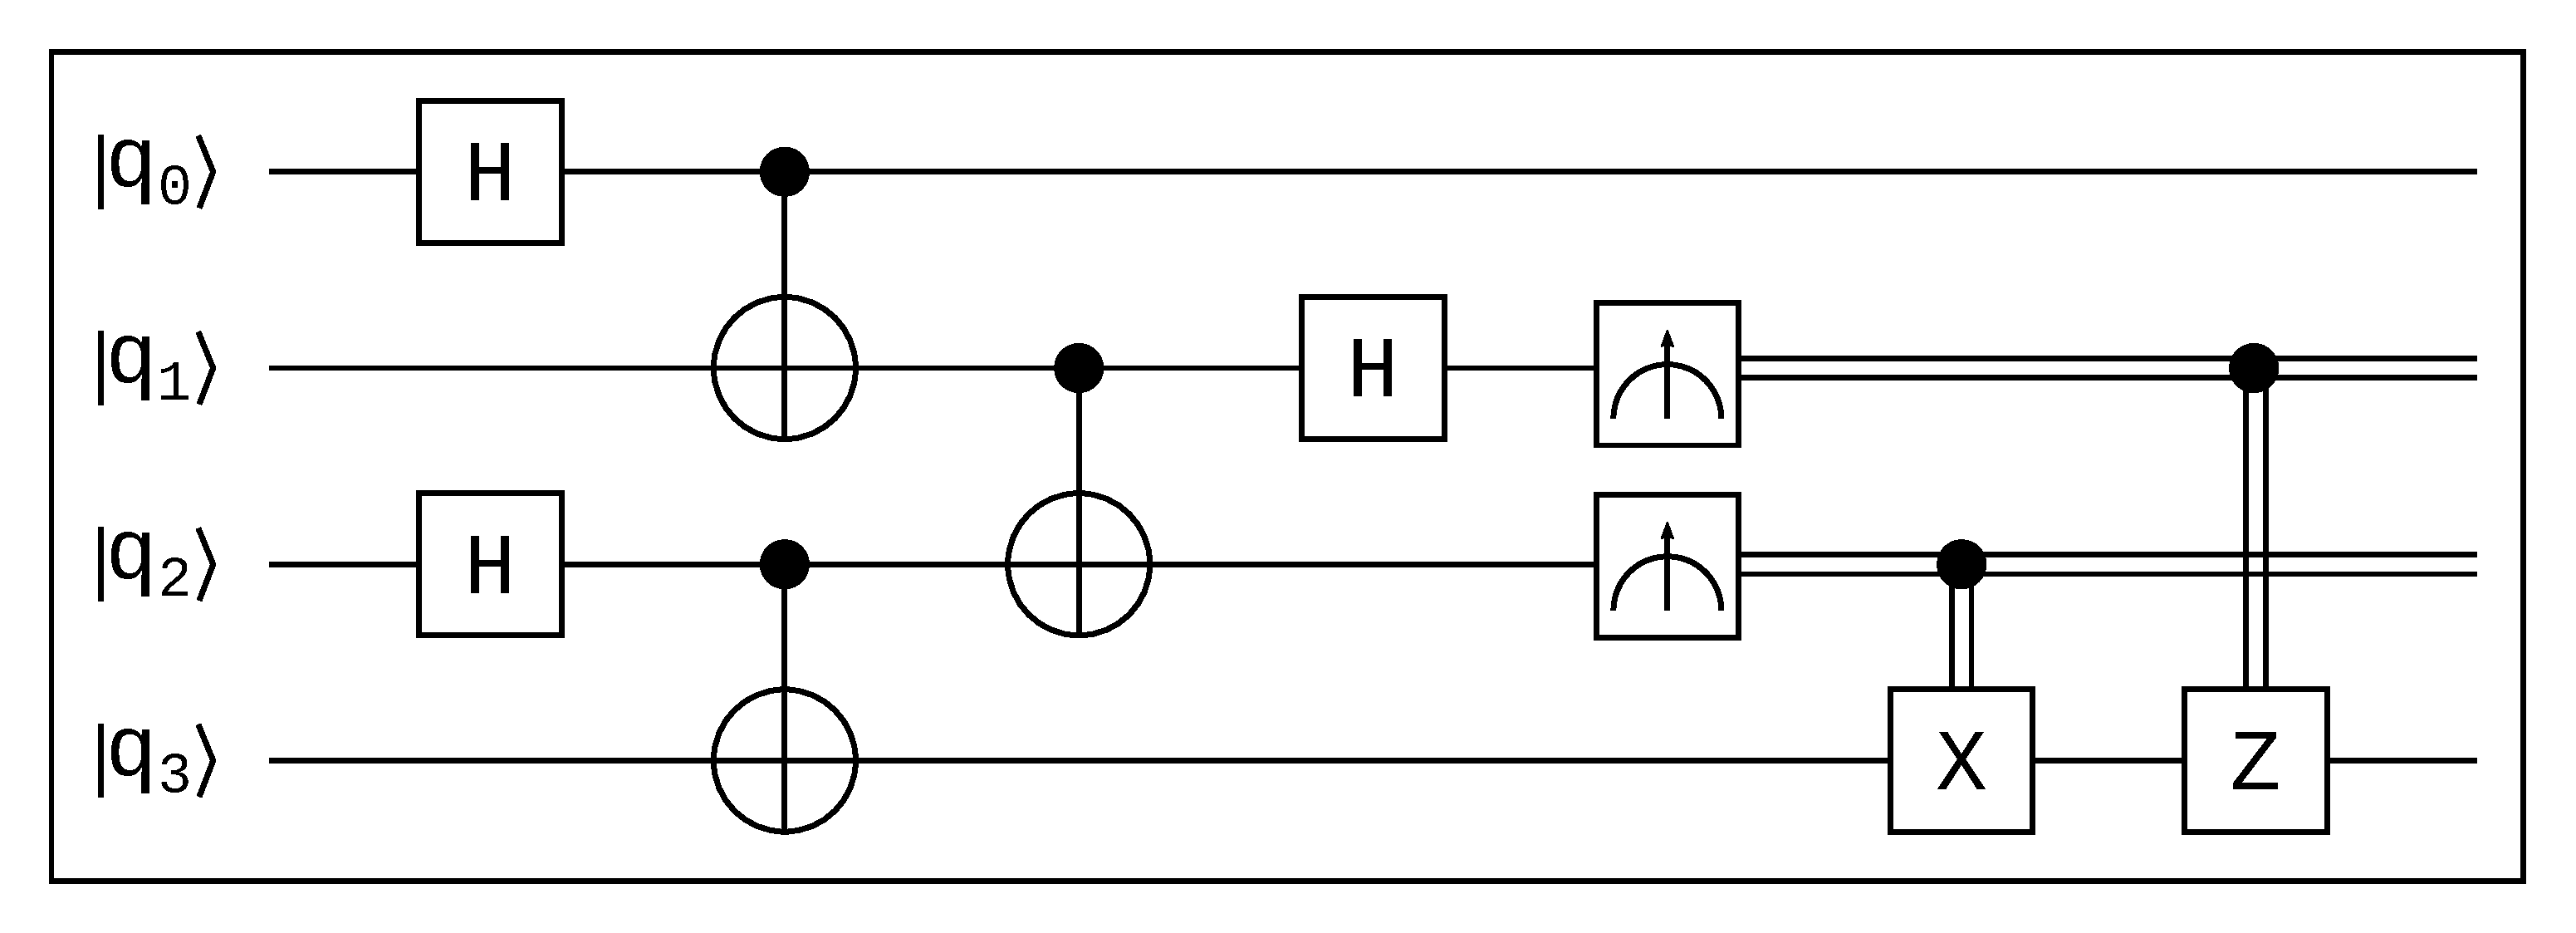
\includegraphics[scale=0.25]{img/qci_a3_question6.ps}}
  \caption{An arbitrary quantum circuit.}
  \label{fig:circuit3}
\end{figure}

\begin{question}
Consider the quantum circuit presented in Figure~\ref{fig:circuit3} and assume $\ket{q_{0}} = \ket{0}$, $\ket{q_{1}} = \ket{0}$, $\ket{q_{2}} = \ket{0}$ and $\ket{q_{3}} = \ket{0}$; hence, $\ket{\psi_{in}} = \ket{0000}$. Determine, by using the Dirac notation, what is the state vector of the quantum circuit just before the partial measurement?
\label{qst:assignment3_6}
\end{question}
{\small
\texttt{Write down your solution here:}
\begin{equation*}
  \begin{split}
    \text Hq_{0}=\frac{1}{\sqrt{2}}(\ket{0000}+\ket{0001})\\
    \text Hq_{2}=\frac{1}{2}(\ket{0000}+\ket{0100}+\ket{0001}+\ket{0101})\\
    \text CNOT_{0,1}=\frac{1}{2}(\ket{0000}+\ket{0100}+\ket{0011}+\ket{0111})\\
    \text CNOT_{2,3}=\frac{1}{2}(\ket{0000}+\ket{1100}+\ket{0011}+\ket{1111})\\
    \text CNOT_{1,2}=\frac{1}{2}(\ket{0000}+\ket{1100}+\ket{0111}+\ket{1011})\\
    \text Hq_{1}=\frac{1}{\sqrt{2}}\cdot\frac{1}{2}(\ket{0000}+\ket{0010}+\ket{1100}+\ket{1110}+\ket{0101}-\ket{0111}+\ket{1001}-\ket{1011})\\
    \ket{\psi}=\frac{1}{2\sqrt{2}}(\ket{0000}+\ket{0010}+\ket{1100}+\ket{1110}+\ket{0101}-\ket{0111}+\ket{1001}-\ket{1011})\\
  \end{split}
\end{equation*}}
\vspace{0.1cm}

\begin{question}
Considering the state vector obtained in Question~\ref{qst:assignment3_6}. What is the probability  $\Prob{q_{3} = 1}$?
\label{qst:assignment3_7}
\end{question}
{\small
\texttt{Write down your solution here:}
\begin{equation*}
  \begin{split}
    \Prob{q_{3} = 1} &= \ket{1001},\ket{1011},\ket{1100},\ket{1110}\\
    \Prob{q_{3} = 1} &= \frac{4\cdot1}{8}=\frac{4}{8}=\frac{1}{2}=50\%
  \end{split}
\end{equation*}}
\vspace{0.1cm}

\begin{question}
Considering the state vector obtained in Question~\ref{qst:assignment3_6}. Assume that the measuring process returned the following values: $M(\ket{q_{2}}) = 1$ and $M(\ket{q_{1}}) = 0$. What is the state vector of the quantum circuit after the described partial measurement? (Note: Remember to renormalize the vector).
\label{qst:assignment3_8}
\end{question}
{\small
\texttt{Write down your solution here:}
\begin{equation*}
  \begin{split}
  \ket{\psi}=\frac{1}{2\sqrt{2}}(\ket{1100}+\ket{0101})\\
  \text normalising \rightarrow(\frac{1}{\sqrt{2}})^2+(\frac{1}{\sqrt{2}})^2=\frac{1}{8}+\frac{1}{8}=\frac{2}{8}=\frac{1}{4}
  \rightarrow\sqrt{\frac{1}{4}}=\frac{1}{2}\\
  2\cdot\frac{1}{2\sqrt{2}}=\frac{1}{\sqrt{2}}\\
  \text {normalised state} \rightarrow \ket{\psi}=\frac{1}{\sqrt{2}}(\ket{1100}+\ket{0101})
  \end{split}
\end{equation*}}
\vspace{0.1cm}

\begin{question}
Considering the state vector and the measurements indicated in Question~\ref{qst:assignment3_8}. What is the final state vector of the quantum circuit after applying the corrections?
\label{qst:assignment3_9}
\end{question}
{\small
\texttt{Write down your solution here:}
\begin{equation*}
  \begin{split}
    \text Xq_{3} = \frac{1}{\sqrt{2}}(\ket{0100}+\ket{1101}\\
    \text{if } q_2 = 1 \implies \text{apply } X \text{ on } q_3\\
    \text{if } q_1 = 1 \implies \text{apply } Z \text{ on } q_3\\
    \text q_1 \neq 1 \implies \text{Z is not being used}\\
    \ket{\psi}=\frac{1}{\sqrt{2}}(\ket{0100}+\ket{1101})
  \end{split}
\end{equation*}}
\vspace{0.1cm}

\begin{question}
Considering the state vector obtained in Question~\ref{qst:assignment3_6}. Assume that the measuring process returned the following values: $M(\ket{q_{2}}) = 1$ and $M(\ket{q_{1}}) = 1$. What is the final state vector of the quantum circuit after applying the corrections? (Note: Remember to renormalize the vector).
\label{qst:assignment3_10}
\end{question}
{\small
\texttt{Write down your solution here:}
\begin{equation*}
  \begin{split}
  \ket{\psi}=\frac{1}{2\sqrt{2}}\ket{1110}-\ket{0111}\\
  \text normalising \rightarrow(\frac{1}{\sqrt{2}})^2+(\frac{1}{\sqrt{2}})^2=\frac{1}{8}+\frac{1}{8}=\frac{2}{8}=\frac{1}{4}
  \rightarrow\sqrt{\frac{1}{4}}=\frac{1}{2}\\
  \text Xq_3 \rightarrow \frac{1}{\sqrt{2}}(\ket{0110}-\ket{1111}\\
  \text Zq_3 \rightarrow \frac{1}{\sqrt{2}}(\ket{0110}+\ket{1111}\\
  \ket{\psi_{final}}=\frac{1}{\sqrt{2}}(\ket{0110}+\ket{1111}
  \end{split}
\end{equation*}}
